\section*{Part 1: Examining the Data}

\begin{taskbox}[Part 1: introduction in the lab manual]
The maternal and fetal ECG signals and the noise signal are given as \texttt{dat1.mecg}, \texttt{dat1.fecg} and \texttt{dat1.noise}, which can be read with the \texttt{load} command in MATLAB. Each file contains a vector named \texttt{recorded}, in mV, with a sampling frequency of 256~Hz. Add these three signals together to obtain a new signal that is, to a good approximation, a sample of a real signal. Then answer the following questions.
\end{taskbox}

\question{1-1}{Plotting the maternal, fetal, noise and mixed signals in the time domain}

\begin{taskbox}
Plot the three signals (maternal, fetal, noise) and the simulated mixed observation signal in the time domain.
\end{taskbox}

The observation signal of Part~1 was built as $x_{\mathrm{mix}}[n] = m[n] + f[n] + \eta[n]$. Figure~\ref{fig:sources} shows a five-second window; the full-record figure is given in the appendix (Figure~\ref{fig:fullsources}). The fetal beats repeat at shorter intervals. Noise and the temporal overlap of beats mean that the peaks visible in the mixture cannot be attributed directly to a single source. Observing the mixture alone is therefore not sufficient for labeling individual peaks.

\begin{figure}[H]
\centering
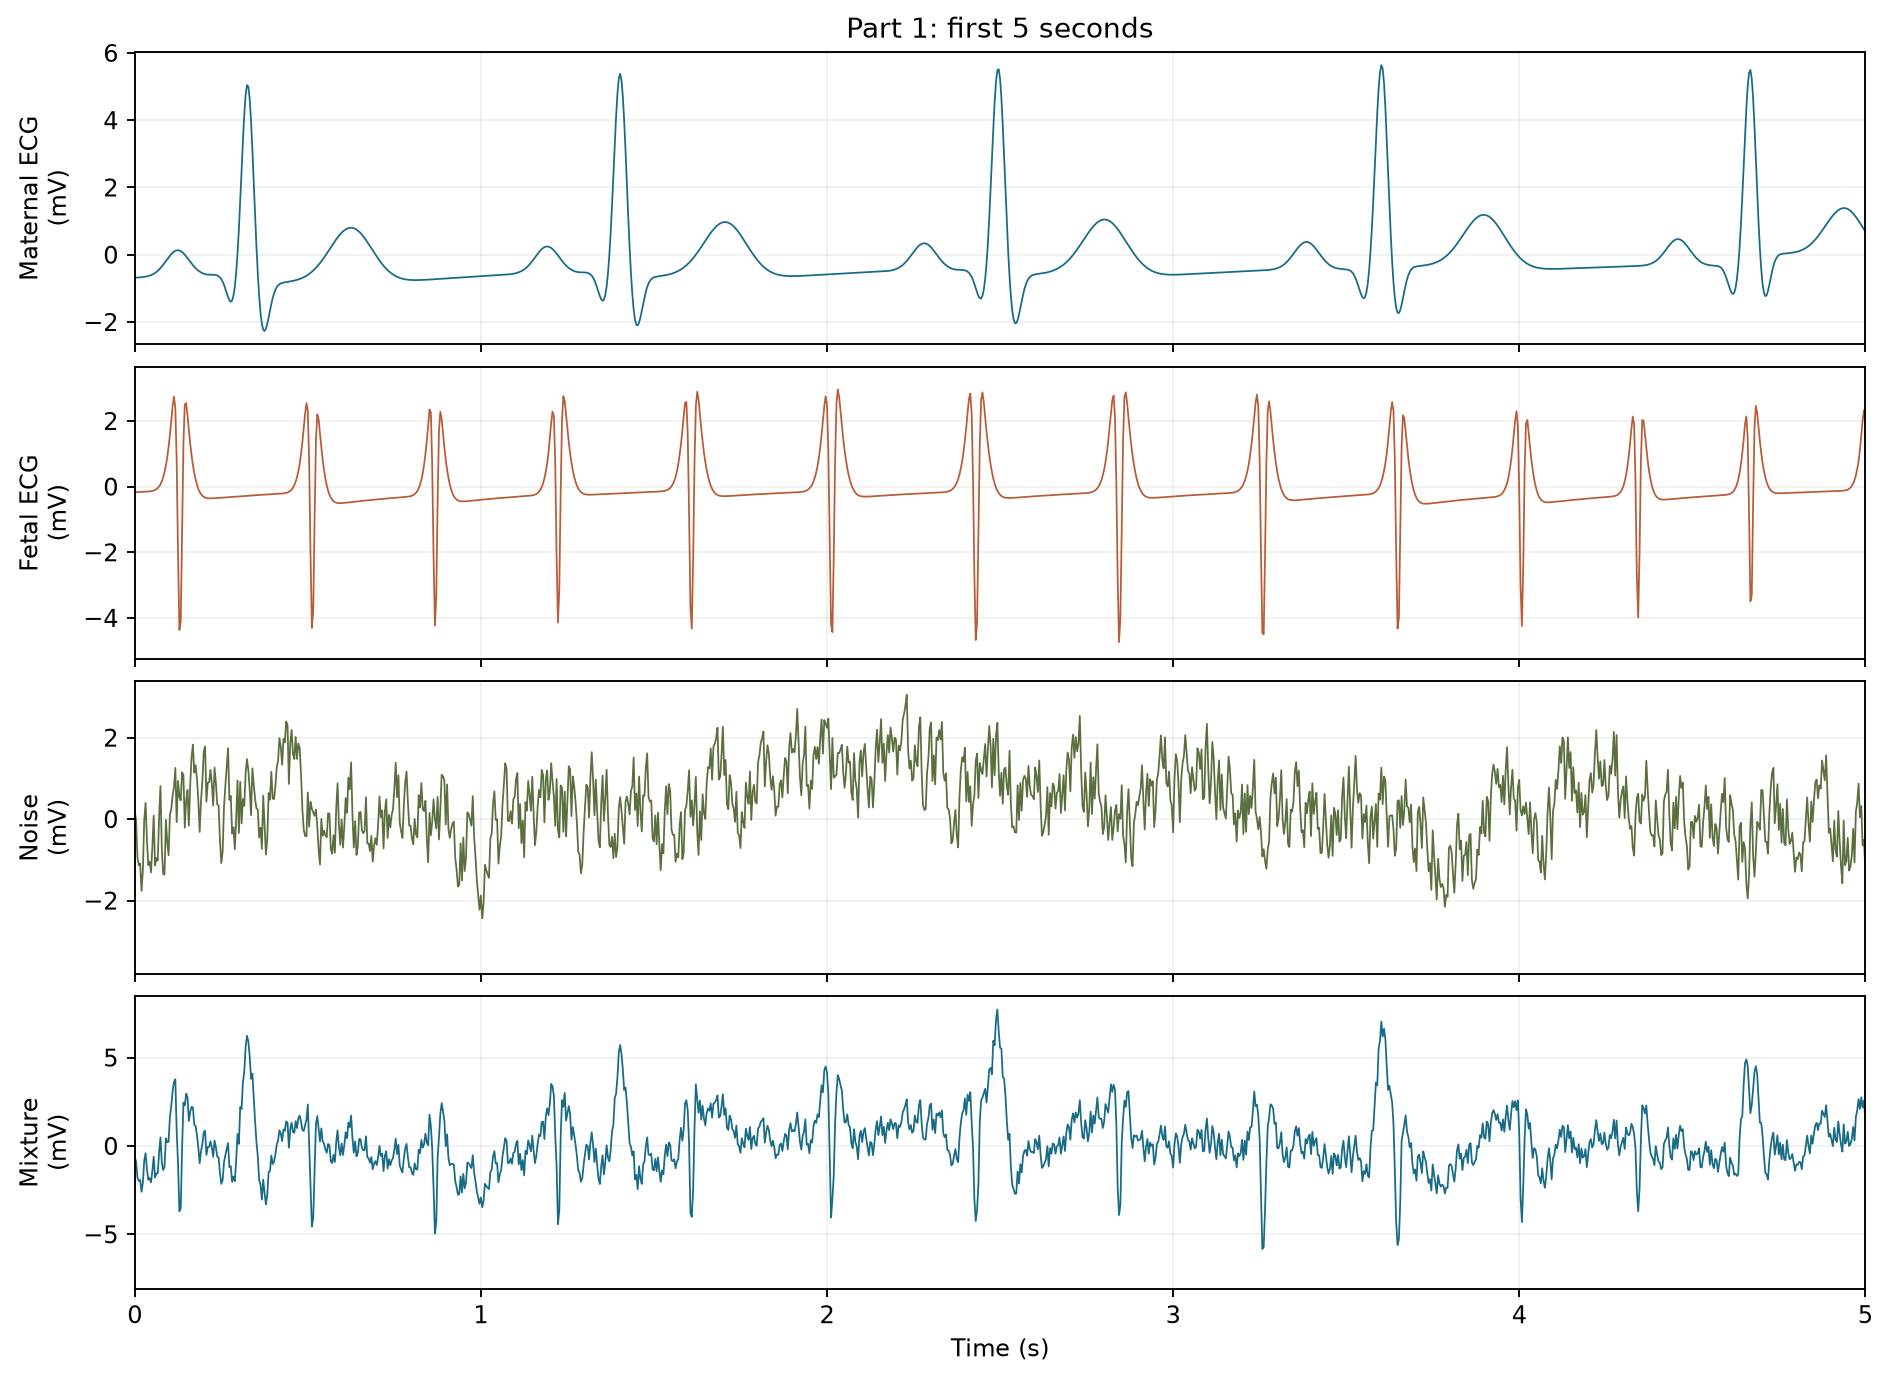
\includegraphics[width=0.8\textwidth]{fig01_time_domain_sources.png}
\caption{Maternal, fetal and noise signals and their sum over the first five seconds.}
\label{fig:sources}
\end{figure}

\question{1-2}{Power spectrum and comparison of frequency content}

\begin{taskbox}
Plot the power spectrum of these three signals using the \texttt{pwelch} command. Are the frequency contents of the maternal and fetal signals comparable? Briefly state the similarities and differences of these frequency contents.
\end{taskbox}

The power spectral density was computed with \texttt{scipy.signal.welch} using a common setup: a symmetric 512-sample Hamming window, an overlap of 256 samples, \texttt{nfft=1024} and \texttt{detrend=False}. The output is one-sided, with density scaling and units of $\mathrm{mV^2/Hz}$. The frequency points are spaced \SI{0.25}{\hertz} apart; zero-padding the FFT does not increase the true resolution of the two-second window.

\begin{figure}[H]
\centering
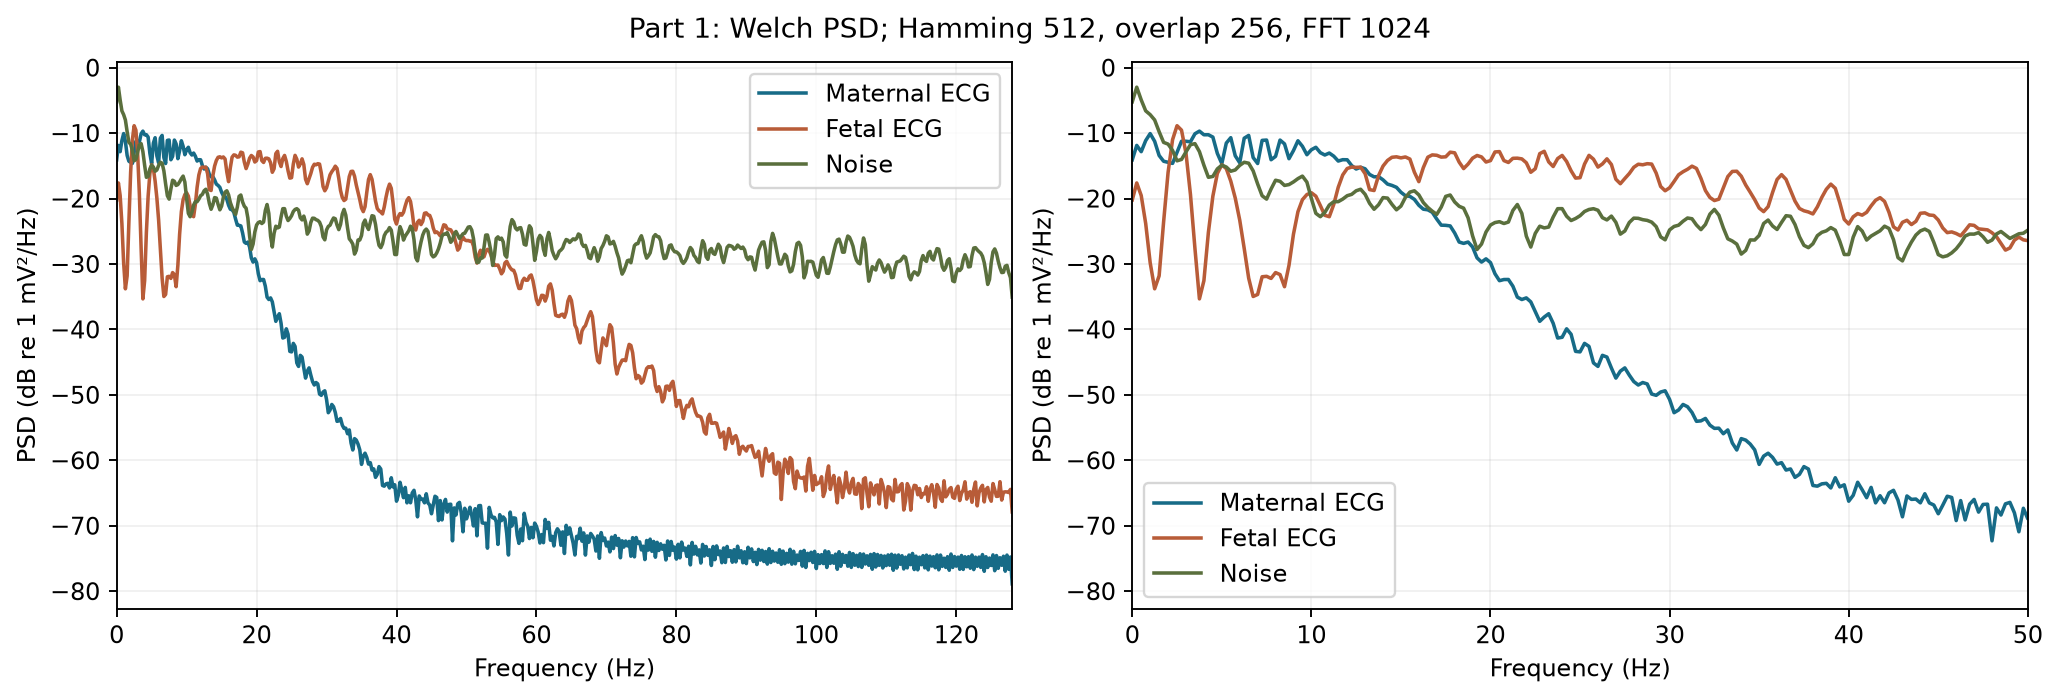
\includegraphics[width=\textwidth]{fig02_welch_psd_sources.png}
\caption{Welch estimates of the sources; left: up to \SI{128}{\hertz}, right: zoomed view up to \SI{50}{\hertz}.}
\label{fig:welch}
\end{figure}

\answer Both ECG signals have low-frequency content and a peaked structure. The maternal spectrum falls off faster beyond about \SI{20}{\hertz}, whereas the fetal content extends to higher frequencies. The noise is broader, and its spectrum is not perfectly flat. The overlap of the two ECG spectra makes a complete separation with a single frequency boundary difficult. This description applies to this dataset only and does not define a fixed band for all ECG signals.


\question{1-3}{Mean, variance and their relation to the spectrum}

\begin{taskbox}
Compute and report the mean and variance of these three signals. Are they comparable? Does the value of the variance have any particular relation to the frequency content of the signals?
\end{taskbox}

The sample mean and sample variance were computed from the following relations:
\begin{equation}
\bar{x} = \frac{1}{M}\sum_{n=1}^{M} x_n,\qquad
s_x^2 = \frac{1}{M-1}\sum_{n=1}^{M}(x_n-\bar{x})^2 .
\label{eq:meanvar}
\end{equation}

\begin{table}[H]
\centering
\caption{Sample mean and variance of the sources of Part 1.}
\begin{tabular}{@{}lrr@{}}
\toprule
\textbf{Source} & \textbf{Mean (mV)} & \textbf{Sample variance (mV$^2$)}\\
\midrule
Maternal & $-2.466172\times10^{-10}$ & 0.999999999\\
Fetal    & $-4.250043\times10^{-10}$ & 1.000000001\\
Noise    & $-4.769102\times10^{-10}$ & 1.000000001\\
\bottomrule
\end{tabular}
\end{table}

The means are practically zero and the variance of all three sources is approximately one, so from this point of view they are comparable. Nevertheless, they have different spectra: the variance expresses the total power around the mean and does not determine where that power lies on the frequency axis. The integral of the one-sided PSD of a centered process is related to its variance; the limited Welch estimate, however, is not necessarily equal to the variance of the whole record, because of windowing and segmentation.

\question{1-4}{Histogram, fourth moment and Gaussianity}

\begin{taskbox}
Compute the histogram of these signals (to approximate the PDF of the components) and include it in your report. Compute the fourth-order moment of these signals using the kurtosis command and report it. Can you tell the degree of Gaussianity of their PDFs from these values?
\end{taskbox}

The histograms were drawn with density normalization, so their areas are approximately one. In Figure~\ref{fig:hist}, the dashed line shows the Gaussian distribution with the same mean and variance as the corresponding source. To avoid confusing the fourth moment with kurtosis, the two definitions below are reported separately:
\begin{equation}
m_4 = \frac{1}{M}\sum_{n}(x_n-\bar{x})^4,\qquad
\beta_2 = \frac{m_4}{\Bigl[\frac{1}{M}\sum_{n}(x_n-\bar{x})^2\Bigr]^{2}} .
\label{eq:kurt}
\end{equation}
Kurtosis was computed with \texttt{scipy.stats.kurtosis} using \texttt{fisher=False} and \texttt{bias=True}. The Gaussian value in this convention is three; the excess kurtosis is therefore $\beta_2-3$.

\begin{table}[H]
\centering
\caption{Fourth central moment, Pearson kurtosis and excess kurtosis.}
\begin{tabular}{@{}lrrr@{}}
\toprule
\textbf{Source} & $m_4$ \textbf{(mV$^4$)} & $\beta_2$ & $\beta_2-3$\\
\midrule
Maternal & 14.031126 & 14.042094 & 11.042094\\
Fetal    &  8.983100 &  8.990122 &  5.990122\\
Noise    &  2.764075 &  2.766235 & $-0.233765$\\
\bottomrule
\end{tabular}
\end{table}

\begin{figure}[H]
\centering
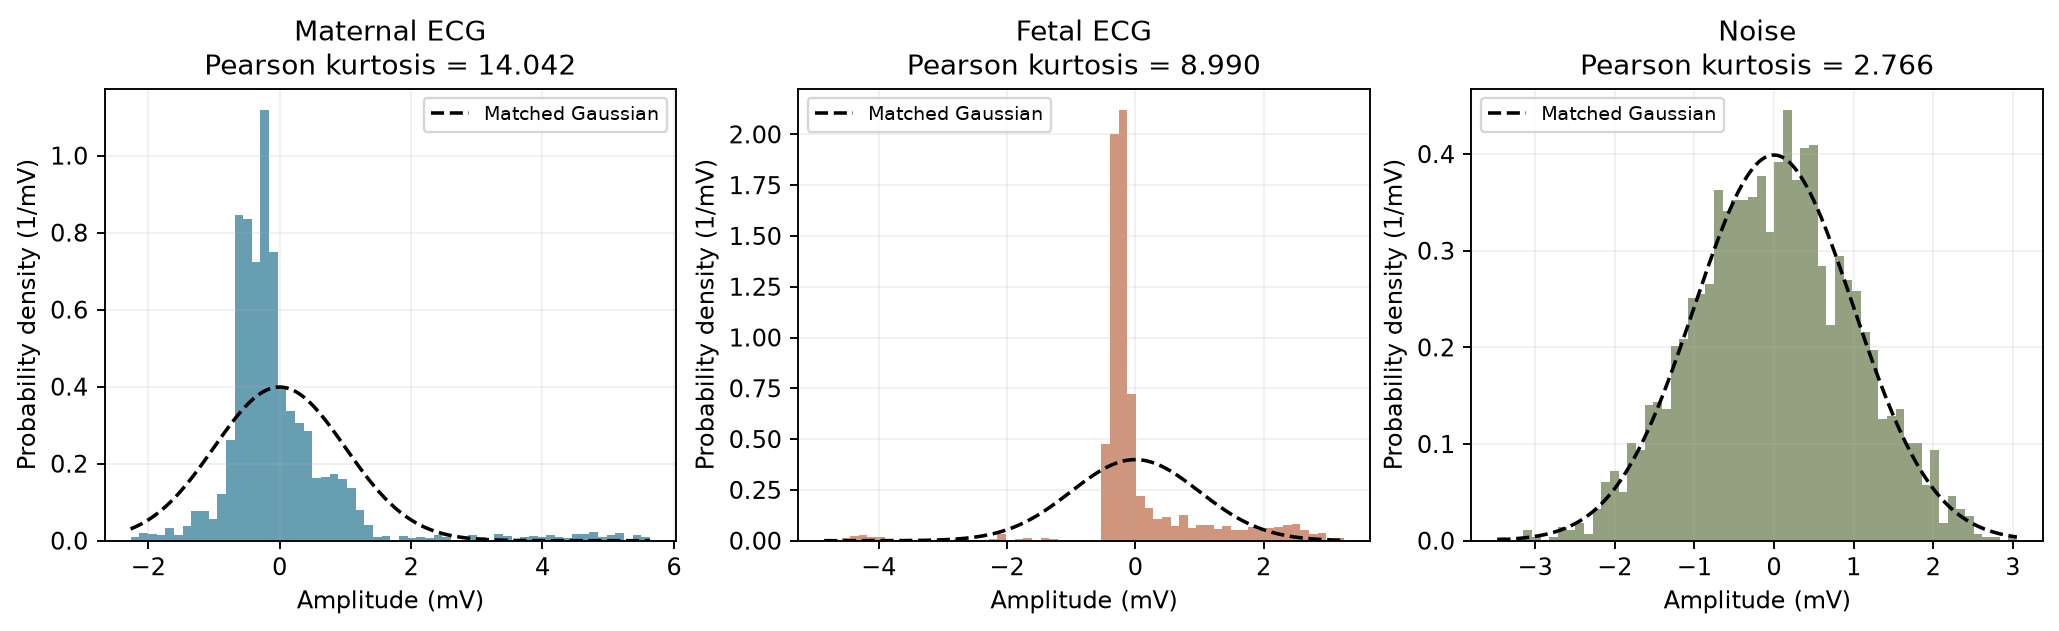
\includegraphics[width=\textwidth]{fig03_histograms_kurtosis.png}
\caption{Approximation of the amplitude density and comparison with a Gaussian of the same mean and variance.}
\label{fig:hist}
\end{figure}

\answer The kurtosis of the maternal and fetal signals is clearly greater than three, and their histograms differ from a Gaussian. The noise, with a value of 2.766235, is closer to three and has a more bell-like shape. A moment being close to its Gaussian value is not proof of Gaussianity: non-Gaussian distributions can also have a kurtosis of three. In this experiment the histogram and kurtosis are descriptive evidence only, and no formal normality test was performed.
